After looking at the advantages and disadvantages of cement batteries, we have brainstormed and established details regarding incorporating cement batteries within a photovoltaic system. First, these batteries will only be installed on the floors and the ceilings. We require additional research and experiments before the feasibility of installing cement batteries in vertical walls can be determined. Therefore, in the following diagram, the battery can be implemented inside the concrete slab, between the insulation layer and damp-proof membrane:
\begin{figure}[H]
\centering
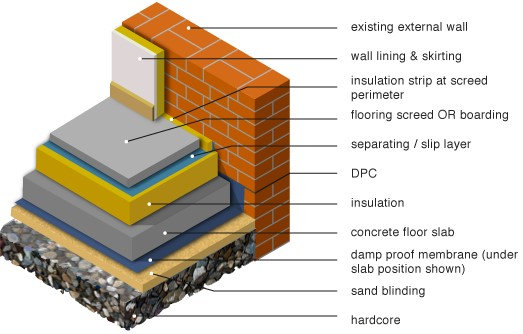
\includegraphics[scale=0.75]{C}
\caption{A breakdown of the structure of concrete floors}\cite{property:floor}
\end{figure}
By having two pieces of uncoated CF as current collectors as presented in Figure~\ref{fig:bat}, we can direct the current through an inverter, which will then supply energy to electric appliances within the house. In addition, the multiple floors and ceilings inside the home will allow more electricity to be stored, thus possibly powering the entire house on its own.